%% LyX 1.3 created this file.  For more info, see http://www.lyx.org/.
%% Do not edit unless you really know what you are doing.
\documentclass[english, 12pt]{article}
\usepackage{times}
%\usepackage{algorithm2e}
\usepackage{url}
\usepackage{bbm}
\usepackage[T1]{fontenc}
\usepackage[latin1]{inputenc}
\usepackage{geometry}
\geometry{verbose,letterpaper,tmargin=2cm,bmargin=2cm,lmargin=1.5cm,rmargin=1.5cm}
\usepackage{rotating}
\usepackage{color}
\usepackage{graphicx}
\usepackage{subcaption}
\usepackage{amsmath, amsthm, amssymb}
\usepackage{setspace}
\usepackage{lineno}
\usepackage{hyperref}
\usepackage{bbm}
\usepackage{makecell}

%\renewcommand{\arraystretch}{1.8}

%\usepackage{xr}
%\externaldocument{SCT-supp}

%\linenumbers
%\doublespacing
\onehalfspacing
%\usepackage[authoryear]{natbib}
\usepackage{natbib} \bibpunct{(}{)}{;}{author-year}{}{,}

%Pour les rajouts
\usepackage{color}
\definecolor{trustcolor}{rgb}{0,0,1}

\usepackage{dsfont}
\usepackage[warn]{textcomp}
\usepackage{adjustbox}
\usepackage{multirow}
\usepackage{graphicx}
\graphicspath{{figures/}}
\DeclareMathOperator*{\argmin}{\arg\!\min}

\let\tabbeg\tabular
\let\tabend\endtabular
\renewenvironment{tabular}{\begin{adjustbox}{max width=0.9\textwidth}\tabbeg}{\tabend\end{adjustbox}}

\makeatletter

%%%%%%%%%%%%%%%%%%%%%%%%%%%%%% LyX specific LaTeX commands.
%% Bold symbol macro for standard LaTeX users
%\newcommand{\boldsymbol}[1]{\mbox{\boldmath $#1$}}

%% Because html converters don't know tabularnewline
\providecommand{\tabularnewline}{\\}

\usepackage{babel}
\makeatother


\begin{document}


\title{Supplementary Materials}

\date{~ }
\maketitle


%%%%%%%%%%%%%%%%%%%%%%%%%%%%%%%%%%%%%%%%%%%%%%%%%%%%%%%%%%%%%%%%%%%%%%%%%%%%%%%%

\renewcommand{\thefigure}{S\arabic{figure}}
\setcounter{figure}{0}
\renewcommand{\thetable}{S\arabic{table}}
\setcounter{table}{0}
\renewcommand{\thesection}{S\arabic{section}}
\setcounter{section}{0}

%%%%%%%%%%%%%%%%%%%%%%%%%%%%%%%%%%%%%%%%%%%%%%%%%%%%%%%%%%%%%%%%%%%%%%%%%%%%%%%%

\section{Designing a reference of allele frequencies from the UK Biobank}

\subsection{Identifying 26 ancestry groups from the UK Biobank}

In this section, we use the first 16 principal components (PCs, \cite{prive2020efficient}) reported by the UK Biobank (Data-Field 22009, \cite{bycroft2018uk}), the self-reported ancestry (Data-Field 21000), and the country of birth (Data-Field 20115).
For the individuals with a missing country of birth, we assign to them ``United Kingdom'' when they self-identify as ``British'' and ``Ireland'' when they self-identify as ``Irish''.
Hereinafter, we use the Euclidean distance based on the first 16 PCs as we have shown to be an appropriate measure of the genetic distance between populations \cite[]{prive2021high}.
The thresholds we use for this distance are based on carefully inspecting the self-reported ancestry and country of birth of individuals kept or excluded.

Since the country of birth may poorly corresponds to the genetic ancestry that we are interested in, we perform some quality control on this information.
Indeed, there are many individuals born in Africa with an Asian self-reported ancestry; we set their country of birth to missing. 
We also set this information to missing for 1/ individuals born outside of Europe that are too close (log-distance lower than 4) to the UK; 2/ individuals born outside the UK within a log-distance of 2.5 to the UK; 3/ individuals born in Europe not within a log-distance of 5 to the UK.
Finally, we keep only individuals born in South Africa with a log-distance to the UK larger than 6 (individuals of African ancestry). 
After applying these filters, there are still many individuals born outside of the UK and Ireland, including e.g.\ 3352 individuals from India, 1100 from Germany, 1036 from Nigeria, and 76 countries with at least 50 individuals.

Then, to define a homogeneous group to be used as a reference population, we choose a country, compute the robust PC center of individuals born in this country (using the geometric median, \cite{prive2021high}), and choose to include in this group all individuals within a chosen log-distance to the center. The distance threshold is chosen based on the countries of birth included.
For groups named after a country, we further restrict to individuals born in this country.
We limit the ancestry groups to 2000 individuals in order not to have very uneven sample sizes; we pick at random among the United Kingdom and Ireland groups.
We manually try different country centers and distance thresholds to cover as much of the worldwide populations as possible, without having overlapping groups.
We also include two other groups: one ``Ashkenazi'' group based on a PC center we defined in \cite{prive2021high}, and a ``South America'' group based on individuals with $\text{PC6} > 50$ and $\text{PC8} < -30$ (clearly separated from the rest of individuals from the UK Biobank). 
Finally, we investigate individuals that are far away from any of the groups defined previously, and add a last group based on a center from remaining individuals born in India.

For each of the 26 ancestry groups we define, we list the individuals' countries of birth (with at least 5 individuals, where ``NA'' means unknown):
\begin{itemize}
\item \textbf{Japan:~~} Japan: 240
\item \textbf{Asia (East):~~} Hong Kong: 390 --- Malaysia: 179 --- NA: 122 --- China: 114 --- Singapore: 58 --- Vietnam: 33 --- Indonesia: 14 --- Taiwan: 10 --- Thailand: 8 --- Brunei: 6 --- Macau (Macao): 6
\item \textbf{Philippines:~~} Philippines: 295
\item \textbf{Africa (South):~~} Zimbabwe: 251 --- Uganda: 57 --- South Africa: 47 --- Zambia: 41 --- Malawi: 10 --- NA: 10 --- Tanzania: 6 --- Congo: 5
\item \textbf{Africa (North):~~} Algeria: 69 --- Morocco: 62 --- Egypt: 54 --- Libya: 36 --- NA: 18 --- Tunisia: 13
\item \textbf{Africa (East 1):~~} Somalia: 81 --- Ethiopia: 58 --- Sudan: 54 --- Eritrea: 46 --- NA: 27
\item \textbf{Africa (East 2):~~} Kenya: 104 --- Uganda: 60 --- Burundi: 18 --- NA: 16 --- Sudan: 14 --- Tanzania: 14 --- Rwanda: 13 --- Nigeria: 8 --- Somalia: 7 --- Angola: 5 --- Zimbabwe: 5
\item \textbf{Caribbean:~~} Caribbean: 327 --- NA: 310 --- Barbados: 73 --- The Guianas: 23 --- Antigua and Barbuda: 7
\item \textbf{Africa (West):~~} Nigeria: 217 --- Ghana: 175 --- NA: 122 --- Sierra Leone: 98 --- Caribbean: 80 --- Ivory Coast: 7 --- Liberia: 7 --- The Guianas: 7 --- Togo: 6
\item \textbf{Africa (Central):~~} Congo: 117 --- Cameroon: 42 --- Nigeria: 33 --- NA: 33 --- Angola: 21 --- Caribbean: 8 --- The Guianas: 7
\item \textbf{Middle East:~~} Iraq: 240 --- Iran: 172 --- Turkey: 55 --- NA: 31 --- Syria: 11
\item \textbf{United Kingdom:~~} United Kingdom: 2000
\item \textbf{Ireland:~~} Ireland: 2000
\item \textbf{Finland:~~} Finland: 143
\item \textbf{Scandinavia:~~} Denmark: 142 --- Norway: 82 --- Sweden: 75 --- NA: 68 --- Germany: 25 --- Netherlands: 17 --- Iceland: 5
\item \textbf{Europe (South West):~~} Spain: 279 --- Portugal: 198 --- NA: 91 --- France: 25 --- Gibraltar: 7
\item \textbf{Italy:~~} Italy: 345
\item \textbf{Europe (South East):~~} NA: 115 --- Romania: 47 --- Serbia/Montenegro: 41 --- Bosnia and Herzegovina: 34 --- Bulgaria: 33 --- Croatia: 28 --- Hungary: 17 --- Italy: 11 --- Macedonia: 8
\item \textbf{Europe (Central):~~} NA: 196 --- Germany: 111 --- Czech Republic: 79 --- Poland: 50 --- Austria: 33 --- Hungary: 27 --- Slovakia: 25 --- Croatia: 10 --- Slovenia: 8 --- France: 7
\item \textbf{Europe (North East):~~} Russia: 88 --- NA: 87 --- Poland: 72 --- Ukraine: 34 --- Latvia: 10 --- Germany: 7 --- Kazakhstan: 6 --- Lithuania: 5
\item \textbf{Pakistan:~~} Pakistan: 400
\item \textbf{Sri Lanka:~~} Sri Lanka: 372
\item \textbf{Bangladesh:~~} Bangladesh: 223
\item \textbf{South America:~~} Colombia: 173 --- Chile: 57 --- Mexico: 51 --- Peru: 50 --- Ecuador: 33 --- Bolivia: 21 --- NA: 20 --- Venezuela: 15 --- Brazil: 10 --- United Kingdom: 8 --- USA: 8 --- Argentina: 5
\item \textbf{Ashkenazi:~~} United Kingdom: 1182 --- NA: 572 --- USA: 115 --- Israel: 27 --- Hungary: 12 --- Ireland: 8 --- France: 7 --- Canada: 6 --- Russia: 5
\item \textbf{India:~~} NA: 258 --- India: 108 --- Sri Lanka: 16 --- Pakistan: 11
\end{itemize}


\subsection{Computing allele frequencies}

We download the 1000 Genomes (1KG) Project data \cite[]{10002015global}. 
Using PLINK \cite[]{chang2015second}, we remove 9 outlier individuals identified in \cite{martin2017human}, filter for founders, non-sex chromosomes, non-multiallelic variants with minor allele counts of at least 10.
From the UK Biobank, we select imputed variants with a minor allele frequency larger than 0.001 and INFO score larger than 0.3, and match these variants with the ones from the filtered 1KG data described previously.
We identify 12,373,666 genetic variants in common, for which we compute allele frequencies for each of the 26 1KG populations. 
We also compute allele frequencies from the BGEN imputed data for each of the 26 UK Biobank groups we identified previously. 

\subsection{Designing the final set of variants}

We select variants with an INFO score of at least 0.4 in all 26 UK Biobank ancestry groups.
Based on the remaining 5,840,630 variants, we compute the overall fixation indices $F_{ST}$ between the UK Biobank groups and the 1KG populations (See the description of the 1KG populations at \url{https://www.coriell.org/1/NHGRI/Collections/1000-Genomes-Collections/1000-Genomes-Project}).
We report all $F_{ST}$ at \url{https://github.com/privefl/freq-ancestry/blob/main/all_fst.csv}, and show only the lowest for each of the 26 ancestry groups we define here:
\begin{itemize}
\item \textbf{Japan:~~} JPT: 0.00033 --- CHB: 0.007 --- CHS: 0.0089 --- Asia (East): 0.01 --- KHV: 0.014 --- CDX: 0.017 --- Philippines: 0.021
\item \textbf{Asia (East):~~} CHS: 0.0009 --- KHV: 0.0021 --- CHB: 0.0029 --- CDX: 0.0034 --- Philippines: 0.01 --- Japan: 0.01 --- JPT: 0.011
\item \textbf{Philippines:~~} Asia (East): 0.01 --- KHV: 0.01 --- CDX: 0.011 --- CHS: 0.012 --- CHB: 0.015 --- Japan: 0.021 --- JPT: 0.021
\item \textbf{Africa (South):~~} Africa (Central): 0.0017 --- LWK: 0.0035 --- Caribbean: 0.0043 --- Africa (West): 0.0044 --- Africa (East 2): 0.005 --- YRI: 0.005 --- ESN: 0.0055
\item \textbf{Africa (North):~~} PUR: 0.01 --- Middle East: 0.01 --- Italy: 0.01 --- Europe (South West): 0.011 --- TSI: 0.012 --- IBS: 0.012 --- Ashkenazi: 0.012
\item \textbf{Africa (East 1):~~} Africa (North): 0.018 --- ASW: 0.027 --- Africa (East 2): 0.028 --- PUR: 0.029 --- Middle East: 0.036 --- ACB: 0.037 --- CLM: 0.039
\item \textbf{Africa (East 2):~~} LWK: 0.0033 --- Caribbean: 0.0045 --- ASW: 0.0048 --- ACB: 0.0048 --- Africa (South): 0.005 --- Africa (Central): 0.0056 --- Africa (West): 0.0074
\item \textbf{Caribbean:~~} ACB: 0.00048 --- Africa (West): 0.0011 --- YRI: 0.0022 --- Africa (Central): 0.0023 --- ESN: 0.0028 --- ASW: 0.003 --- MSL: 0.0042
\item \textbf{Africa (West):~~} YRI: 0.00061 --- Caribbean: 0.0011 --- ESN: 0.0015 --- Africa (Central): 0.0019 --- ACB: 0.0023 --- MSL: 0.0028 --- Africa (South): 0.0044
\item \textbf{Africa (Central):~~} Africa (South): 0.0017 --- Africa (West): 0.0019 --- Caribbean: 0.0023 --- YRI: 0.0024 --- ESN: 0.0028 --- ACB: 0.0036 --- LWK: 0.0045
\item \textbf{Middle East:~~} Italy: 0.0043 --- TSI: 0.0059 --- Europe (South East): 0.007 --- Ashkenazi: 0.007 --- Europe (South West): 0.008 --- India: 0.0088 --- IBS: 0.0089
\item \textbf{United Kingdom:~~} Scandinavia: 0.00043 --- Ireland: 0.00069 --- CEU: 0.001 --- GBR: 0.0011 --- Europe (Central): 0.0012 --- Europe (South East): 0.0021 --- Europe (South West): 0.0023
\item \textbf{Ireland:~~} United Kingdom: 0.00069 --- Scandinavia: 0.0015 --- GBR: 0.0017 --- CEU: 0.0018 --- Europe (Central): 0.0023 --- Europe (South West): 0.0033 --- Europe (South East): 0.0033
\item \textbf{Finland:~~} FIN: 0.00041 --- Europe (North East): 0.0052 --- Scandinavia: 0.0054 --- Europe (Central): 0.0056 --- United Kingdom: 0.0066 --- CEU: 0.0067 --- GBR: 0.0072
\item \textbf{Scandinavia:~~} United Kingdom: 0.00043 --- Europe (Central): 0.0012 --- CEU: 0.0013 --- Ireland: 0.0015 --- GBR: 0.0015 --- Europe (South East): 0.0026 --- Europe (North East): 0.0027
\item \textbf{Europe (South West):~~} IBS: 0.00079 --- Italy: 0.0014 --- Europe (South East): 0.002 --- TSI: 0.0021 --- United Kingdom: 0.0023 --- Europe (Central): 0.003 --- CEU: 0.003
\item \textbf{Italy:~~} TSI: 0.0011 --- Europe (South West): 0.0014 --- Europe (South East): 0.0017 --- IBS: 0.0023 --- Europe (Central): 0.004 --- United Kingdom: 0.0041 --- Middle East: 0.0043
\item \textbf{Europe (South East):~~} Europe (Central): 0.00075 --- Italy: 0.0017 --- Europe (North East): 0.0017 --- Europe (South West): 0.002 --- United Kingdom: 0.0021 --- Scandinavia: 0.0026 --- TSI: 0.0027
\item \textbf{Europe (Central):~~} Europe (North East): 0.00053 --- Europe (South East): 0.00075 --- Scandinavia: 0.0012 --- United Kingdom: 0.0012 --- CEU: 0.0019 --- GBR: 0.0023 --- Ireland: 0.0023
\item \textbf{Europe (North East):~~} Europe (Central): 0.00053 --- Europe (South East): 0.0017 --- Scandinavia: 0.0027 --- United Kingdom: 0.003 --- CEU: 0.0036 --- Ireland: 0.0039 --- GBR: 0.0039
\item \textbf{Pakistan:~~} PJL: 0.0026 --- India: 0.0041 --- GIH: 0.0053 --- Bangladesh: 0.0059 --- Sri Lanka: 0.0065 --- ITU: 0.0068 --- STU: 0.0074
\item \textbf{Sri Lanka:~~} STU: 0.00034 --- ITU: 0.0015 --- Bangladesh: 0.0023 --- BEB: 0.0025 --- PJL: 0.0037 --- GIH: 0.0043 --- Pakistan: 0.0065
\item \textbf{Bangladesh:~~} BEB: 0.00068 --- Sri Lanka: 0.0023 --- STU: 0.0028 --- ITU: 0.003 --- PJL: 0.0037 --- GIH: 0.0044 --- Pakistan: 0.0059
\item \textbf{South America:~~} MXL: 0.0023 --- CLM: 0.0053 --- PUR: 0.014 --- PEL: 0.019 --- India: 0.022 --- Pakistan: 0.027 --- Europe (South East): 0.029
\item \textbf{Ashkenazi:~~} Italy: 0.0051 --- TSI: 0.0064 --- Europe (South West): 0.0069 --- Middle East: 0.007 --- Europe (South East): 0.0072 --- IBS: 0.008 --- Europe (Central): 0.0097
\item \textbf{India:~~} Pakistan: 0.0041 --- PJL: 0.007 --- Middle East: 0.0088 --- Europe (South East): 0.0091 --- Bangladesh: 0.0095 --- Europe (Central): 0.0096 --- United Kingdom: 0.0097
\end{itemize}

For each of the 1KG populations, we identify the closest ancestry group among those we defined, compute the $F_{ST}$ for all variants and scale them by dividing by the overall $F_{ST}$ with this group.
For each variant, we then sum these scaled $F_{ST}$ (one for each 1KG population), and identify and remove 24,040 variants with a large score.
This enable us to identify variants with possible errors in the UK Biobank.

\subsection{Designing the final set of reference populations}

The 26 ancestry groups defined previously comprise a total of 15,645 individuals from the UK Biobank. We combine them with 2490 individuals from the 26 populations of the 1KG data, and use a pruned set of 252,893 high-quality genotyped variants to run an admixture analysis (K = 15) using function \texttt{snmf} from R package LEA \cite[]{frichot2014fast,gain2020lea}.
Ancestry proportions for the 52 groups are represented in Figure \ref{fig:admixture}.
We can see that we have defined very homogeneous groups; however based on these results and previous $F_{ST}$, we decide to slightly modify these groups.
First, for the Finland, Bangladesh and Japan ancestry groups, we compute a weighted average of allele frequencies with the ones from the 1KG data (FIN, BEB and JPT) to increase the small sample size of these groups.
We do the same for ``South America'' and ``PEL'' in order to capture slightly more of what is probably an Amerindian ancestral component (in blue).
Second, we merge the ``Irish'' and ``United Kingdom'' groups as a new ``British-Irish Isles'' group.
Third, we remove some groups that could be retrieved from combining two or three other groups: ``Africa (East 2)'', ``Caribbean'', ``Africa (Central)'', ``Scandinavia'', ``Italy'', ``Europe (South East)'', ``Europe (Central)'', and ``India''.

\begin{figure}[hp]
	\centerline{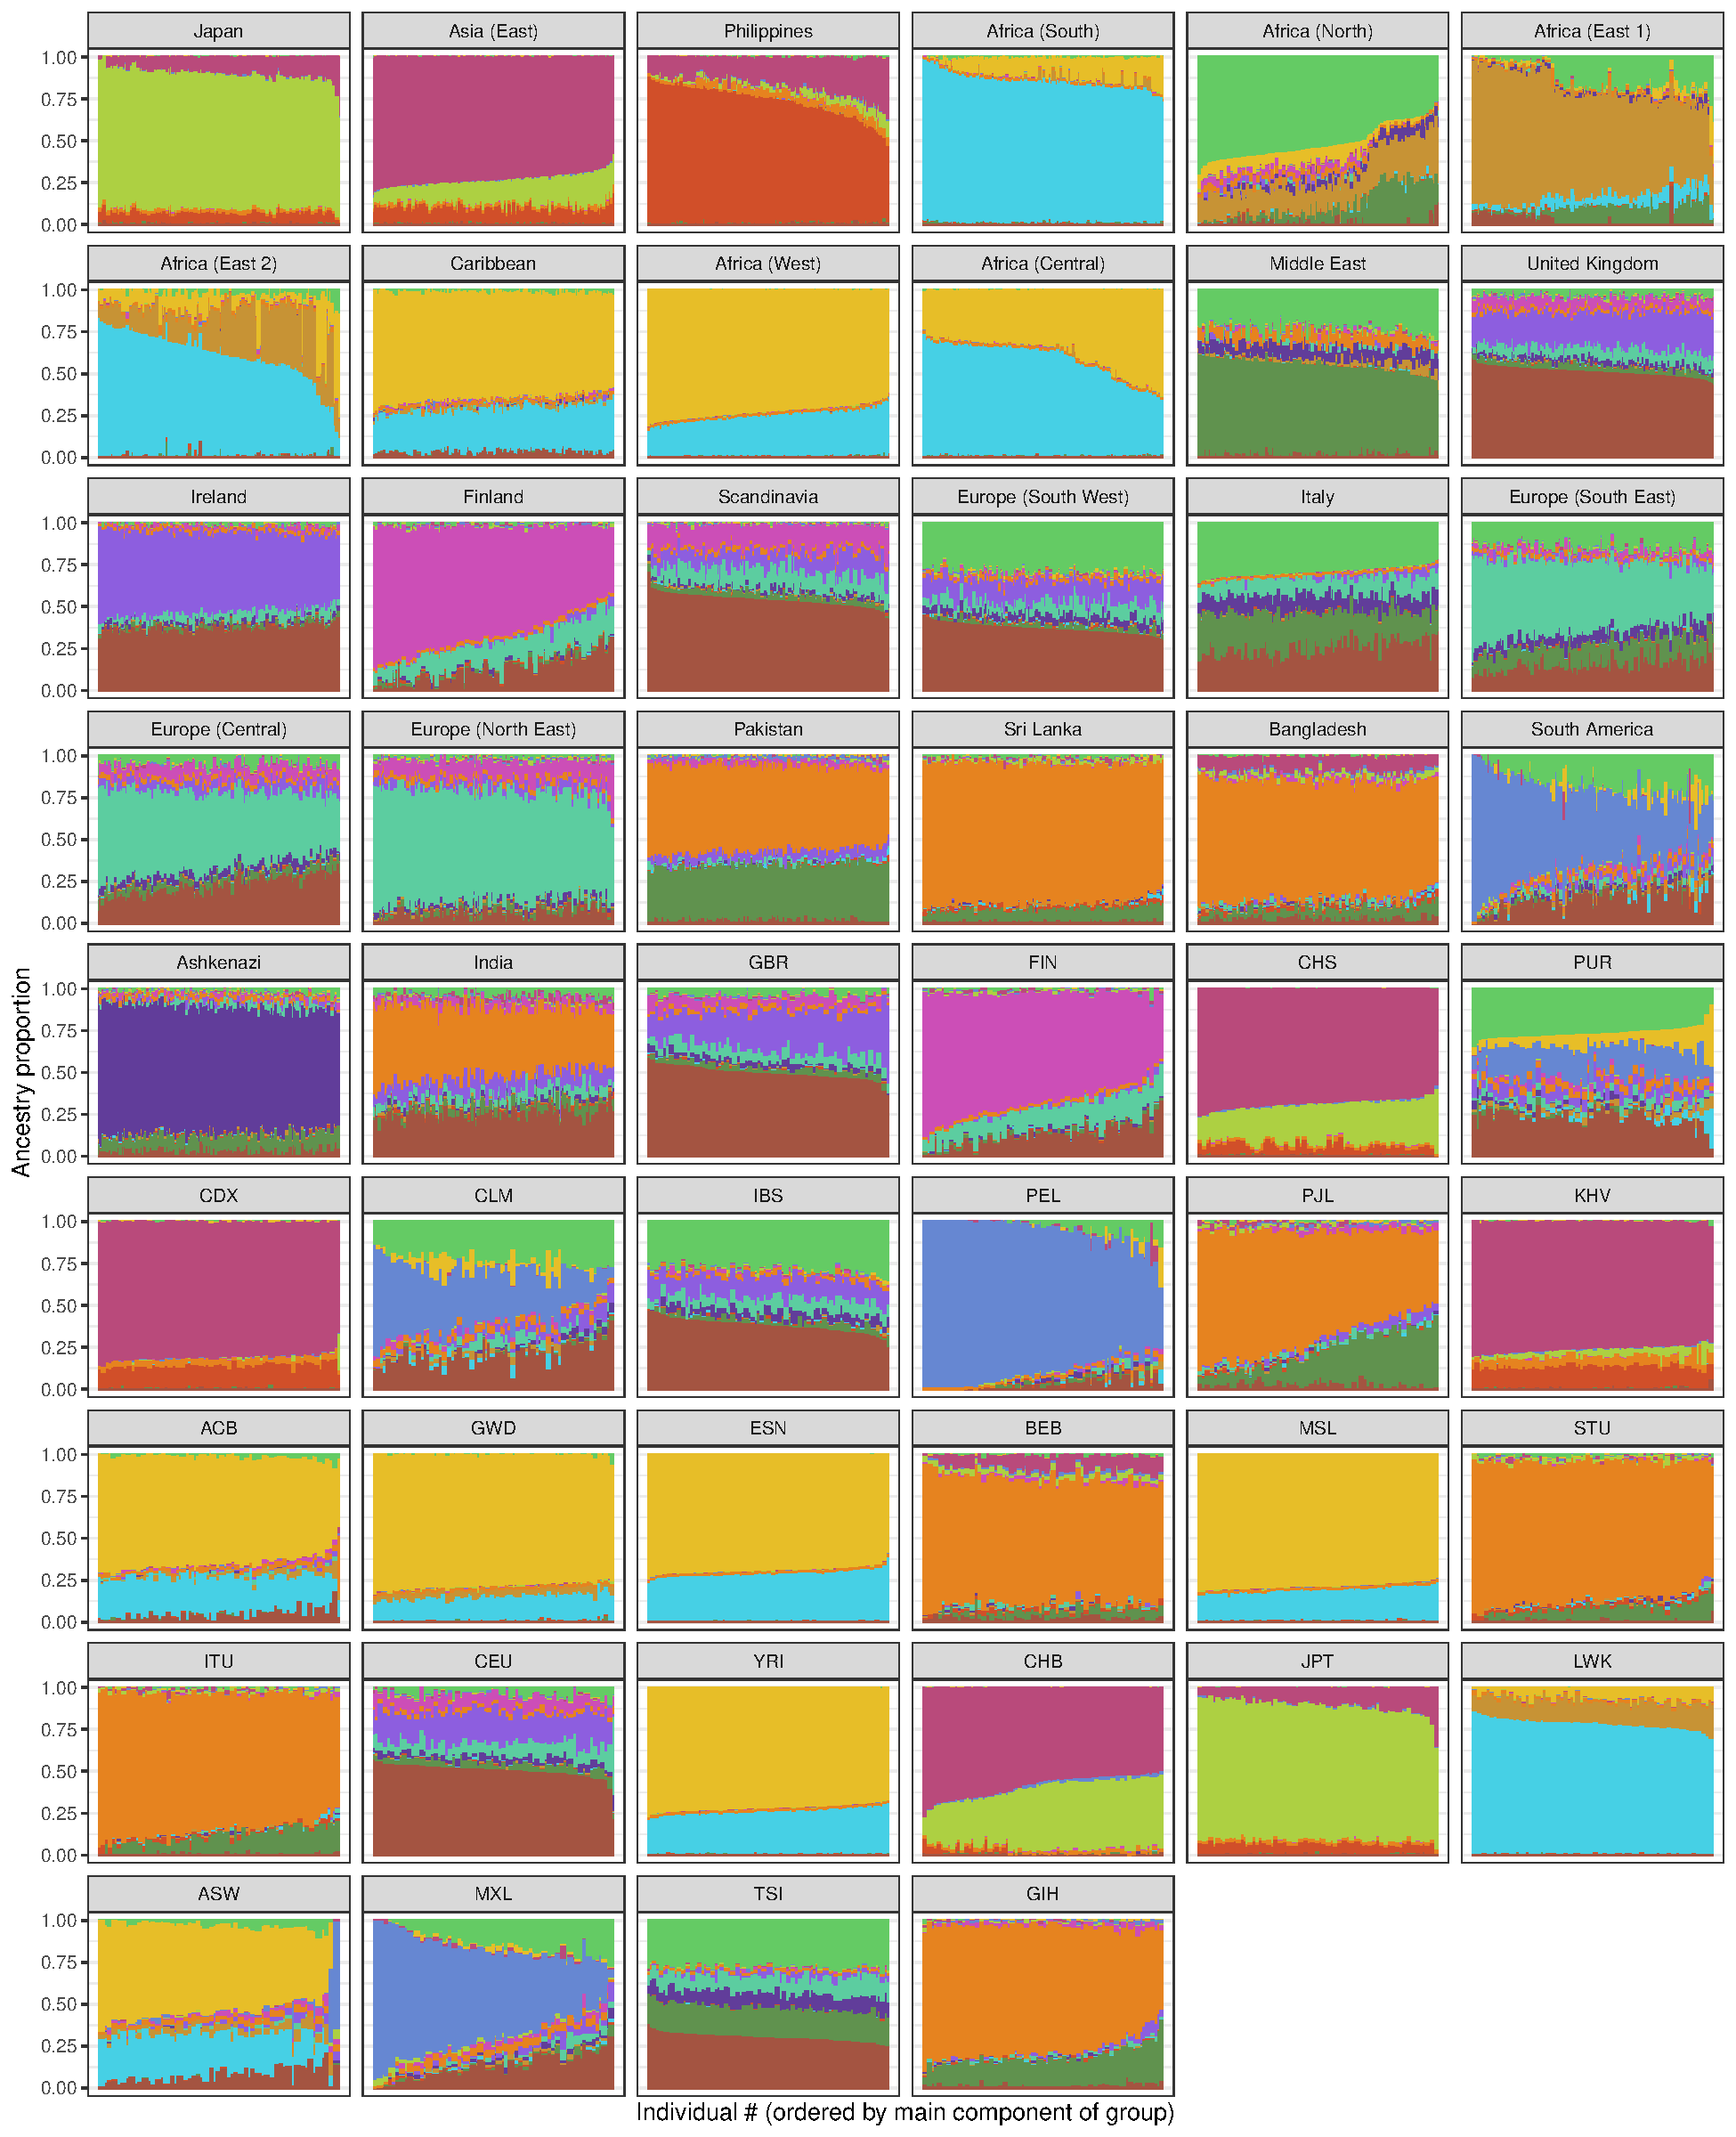
\includegraphics[width=0.92\textwidth]{admixture}}
	\caption{Admixture coefficients (for K = 15 ancestral populations) for the individuals from the 26 ancestry groups we defined previously from the UK Biobank, as well as the 26 1KG populations. \label{fig:admixture}}
\end{figure}

This results in the set of 5,816,590 variants for 17 ancestry groups, which we provide for download and use to estimate ancestry proportions in GWAS summary statistics.

%%%%%%%%%%%%%%%%%%%%%%%%%%%%%%%%%%%%%%%%%%%%%%%%%%%%%%%%%%%%%%%%%%%%%%%%%%%%%%%%

\bibliographystyle{natbib}
\bibliography{refs}

%%%%%%%%%%%%%%%%%%%%%%%%%%%%%%%%%%%%%%%%%%%%%%%%%%%%%%%%%%%%%%%%%%%%%%%%%%%%%%%%

\end{document}
